\documentclass[12pt]{report}

\usepackage[english]{babel}
\usepackage[utf8x]{inputenc}
\usepackage{amsmath}
\usepackage{graphicx}
\usepackage{multirow}
\usepackage[hypcap]{caption}
\usepackage{setspace} 
\usepackage{float}

\title{Lab 3: Strengthening Mechanisms and Aluminum Alloys}
\author{Zachary Tschirhart \\
	\small \\
        \small EID: zst75 \\
	\small Department of Aerospace Engineering and Engineering Mechanics \\
	\small \textbf{ASE 324L (Mon 2:00-5:00)} \\
	\small Unique: 13740}

\date{February 10, 2014}


\begin{document}
\maketitle

\begin{abstract}
In this experiment, several differently treated mixed copper and aluminum specimen were tested in order to find attractive properties for specific purposes. Of the specimens that were tested, the anealed aluminum provided the worst performance of all the materials and had no useful augmented properties for almost any known engineering application. In the case of using the specimen for an aircraft structure, the aluminum treated for two hours displayed the greatest increase in useful properties. In order to compare a single attribute in strength hardening, the amount of precipitate formed in the material was the only varied property in this case. In general, heat treating the specimen increased the strength, but toughness and other properties seemed to vary for each case.

\end{abstract}


\tableofcontents
\pagebreak

\setcounter{secnumdepth}{0}



\section{Introduction}
\doublespacing
Understanding the trade-offs and augmentations that processes can provide materials is important in the engineering field. This knowledge can help optimize the performance of many applications. For example, the structure of an aircraft needs to be both light weight, tough, and strong. The only way this combination can be achieved is by using a small subset of materials that fall in that category. By using different processes to increase these attributes in the material, optimizations can be made and thus more efficient aircraft can be created. In this lab, a series of treated aluminum specimens are tested to find the best combination of properties for the specific application. 


\section{Experimental and Data Reduction Procedures}

The experiment consisted of loading each specimen into the grips of the electromechanical test machine after measuring the diameter and gage length. The gage length had a two inch mark to determine the change in length of the specimen after loading. The machine loaded the specimen by constantly increasing the load over the course of time, until the specimen failed. The data was then compiled and sent for post processing.

When reducing the data, there were a series of equations to calculate the appropriate values. There is a linear relationship between the stress and strain of the test specimen and can be used to find Young's Modulus of the material.

\begin{equation}
\begin{split}
  E = \frac{\sigma}{\varepsilon}
  \label{equation:equation1}
\end{split}
\end{equation}
\\

Where E is Young's modulus, \( \sigma \) is the stress, and \( \varepsilon \) is the strain. This equation can only be used in the linearly elastic region in the stress-strain diagram. 

When looking for Poisson's ratio, only the transverse and axial strain is needed to calculate using the following equation:

\begin{equation}
\begin{split}
  \nu = -\frac{\varepsilon_T}{\varepsilon_a}
  \label{equation:equation2}
\end{split}
\end{equation}
\\

Where \( \nu \) is Poisson's ratio, \(\varepsilon_T\) is the transverse strain, and \(\varepsilon_a\) is the axial strain. 

Then when calculating the toughness of the material, the following equation was needed:

\begin{equation}
\begin{split}
  T = \int_0^{\varepsilon_f} \sigma d\varepsilon
  \label{equation:equation3}
\end{split}
\end{equation}
\\

Where \( \varepsilon_f \) is the stress at failure, \( \sigma \) is the stress, and \( d\varepsilon \) is the differential piece of strain of which the integration is taking place over. 

The first step in analyzing and processing the data is to plot the stress-strain diagram for each type of treated aluminum, showing the difference in cross-head displacement and extensometer data. Each of the figures are shown below, along with the 0.2\% offset to find the yield stress. 

\begin{figure}[H]
	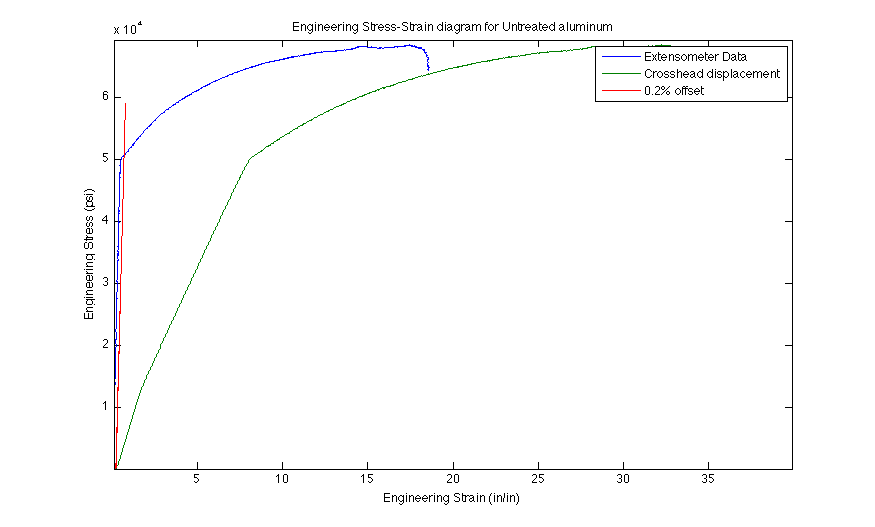
\includegraphics[width=1\textwidth]{untreated-stressvsstrain.png}
	\caption{Engineering stress vs. strain for untreated aluminum with cross-head displacement and extensometer data}
	\label{fig:Figure1}
\end{figure}

\begin{figure}[H]
	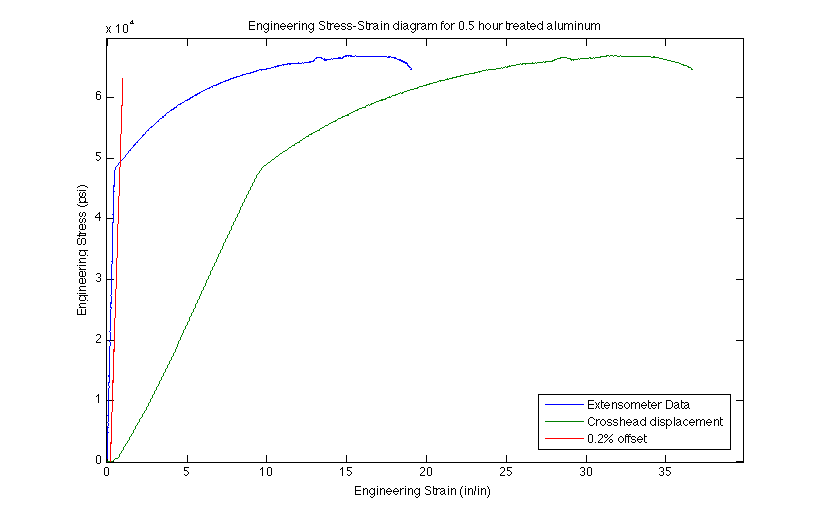
\includegraphics[width=1\textwidth]{thirtymin-stressvsstrain.png}
	\caption{Engineering stress vs. strain for 30 minute treated aluminum with cross-head displacement and extensometer data}
	\label{fig:Figure2}
\end{figure}

\begin{figure}[H]
	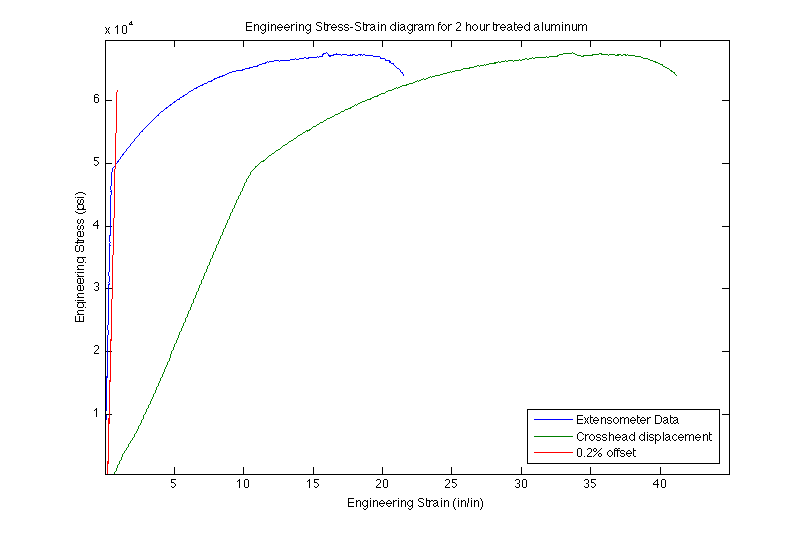
\includegraphics[width=1\textwidth]{2hour-stressvsstrain.png}
	\caption{Engineering stress vs. strain for 2 hour treated aluminum with cross-head displacement and extensometer data}
	\label{fig:Figure3}
\end{figure}

\begin{figure}[H]
	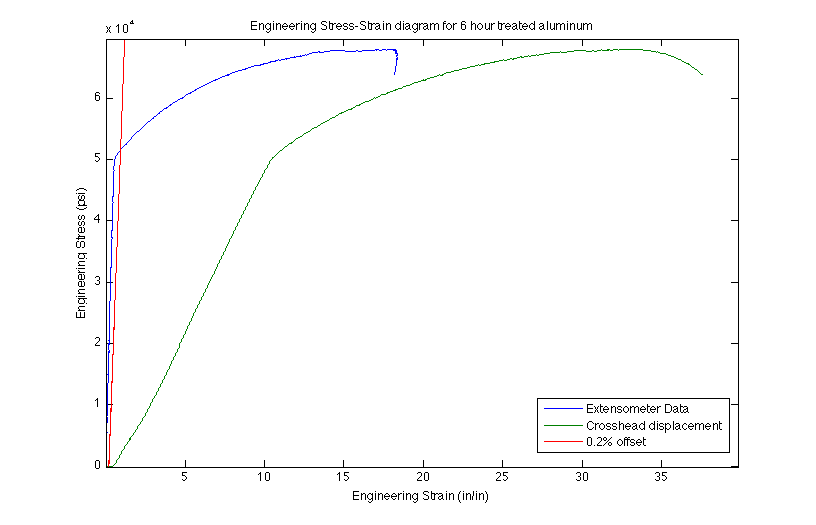
\includegraphics[width=1\textwidth]{6hour-stressvsstrain.png}
	\caption{Engineering stress vs. strain for 6 hour treated aluminum with cross-head displacement and extensometer data}
	\label{fig:Figure4}
\end{figure}

\begin{figure}[H]
	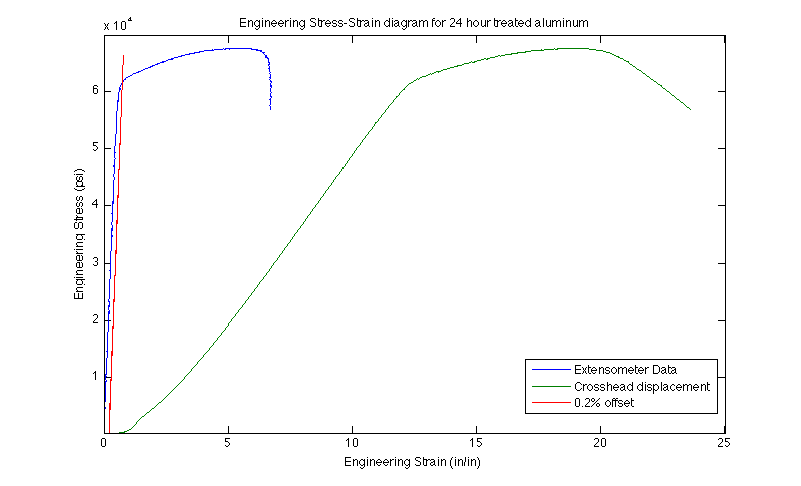
\includegraphics[width=1\textwidth]{24hour-stressvsstrain.png}
	\caption{Engineering stress vs. strain for 24 hour treated aluminum with cross-head displacement and extensometer data}
	\label{fig:Figure5}
\end{figure}

\begin{figure}[H]
	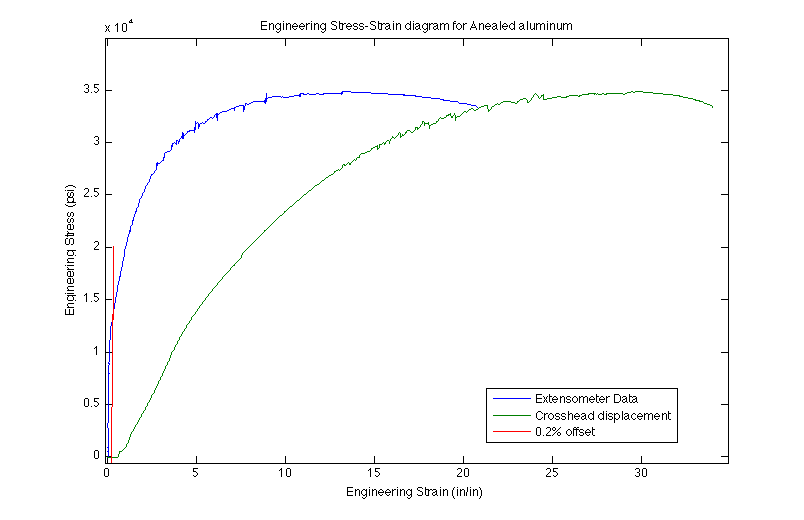
\includegraphics[width=1\textwidth]{anealed-stressvsstrain.png}
	\caption{Engineering stress vs. strain for anealed aluminum with cross-head displacement and extensometer data}
	\label{fig:Figure6}
\end{figure}

As can be seen in figures one through six, the cross-head displacement measures much larger displacements than the extensometer does. This is because the cross-head measurement is taking into account the total displacement of the whole loading device and the specimen, while the extensometer is only measuring the displacement of the specimen. 

In each of these graphs, almost all of the necessary measurements can be found by finding the appropriate values. The only value not calculated by these graphs is the Poisson's Ratio, which is found in the engineering strain vs. strain in the next section. 

\begin{figure}[H]
	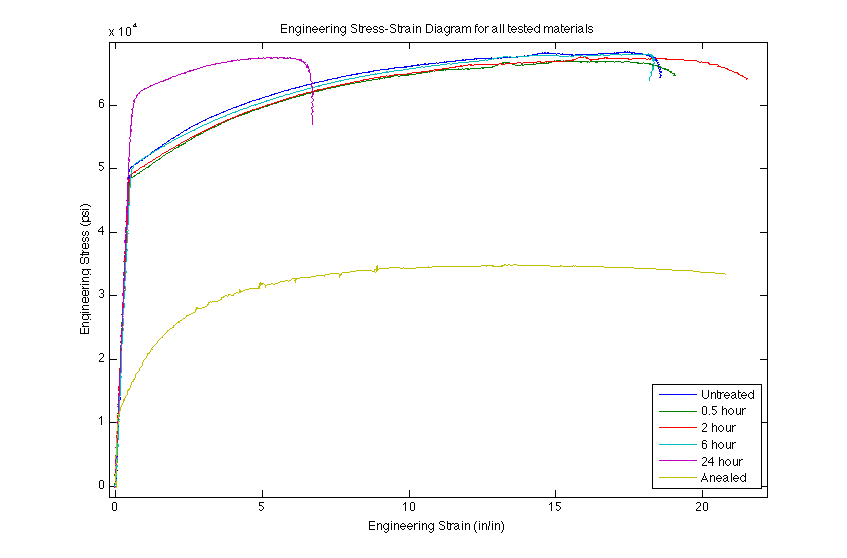
\includegraphics[width=1\textwidth]{all-stressvsstrain.png}
	\caption{Engineering stress vs. strain for all tested materials using extensometer data}
	\label{fig:Figure7}
\end{figure}

Figure 7 shows a visual comparison of all of the tested materials, where there are very clear differences for each of them.

\section{Results and Discussion}
\doublespacing

Most of the figures used to calculate the necessary values are covered in the previous section, although in order to find Poisson's Ratio the axial vs. transverse strain plots are needed. Figures eight through thirteen are the plots needed, with a linear regression to illustrate the linearity of the plot.

\begin{figure}[H]
	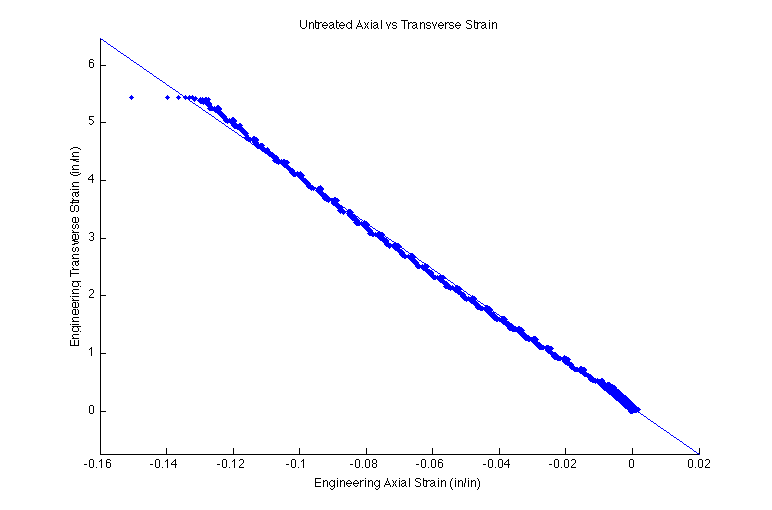
\includegraphics[width=1\textwidth]{untreated-strainvsstrain.png}
	\caption{Engineering axial vs. transverse strain for untreated aluminum}
	\label{fig:Figure8}
\end{figure}

\begin{figure}[H]
	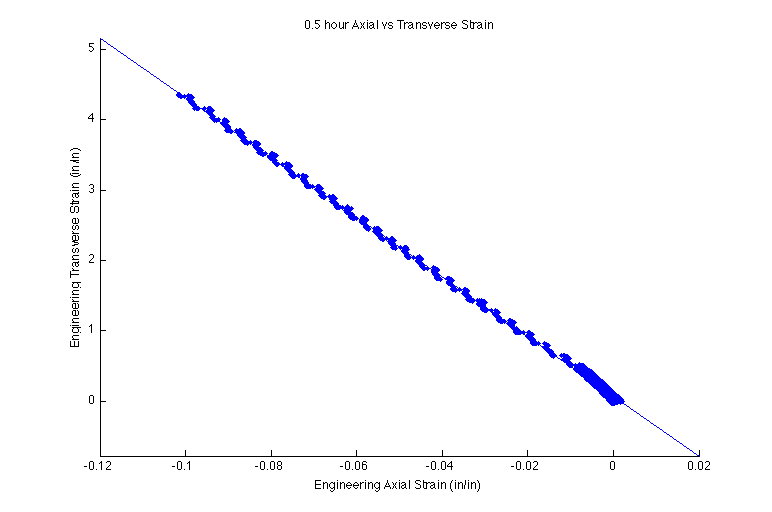
\includegraphics[width=1\textwidth]{thirtymin-strainvsstrain.png}
	\caption{Engineering axial vs. transverse strain for 0.5 hour treated aluminum}
	\label{fig:Figure9}
\end{figure}

\begin{figure}[H]
	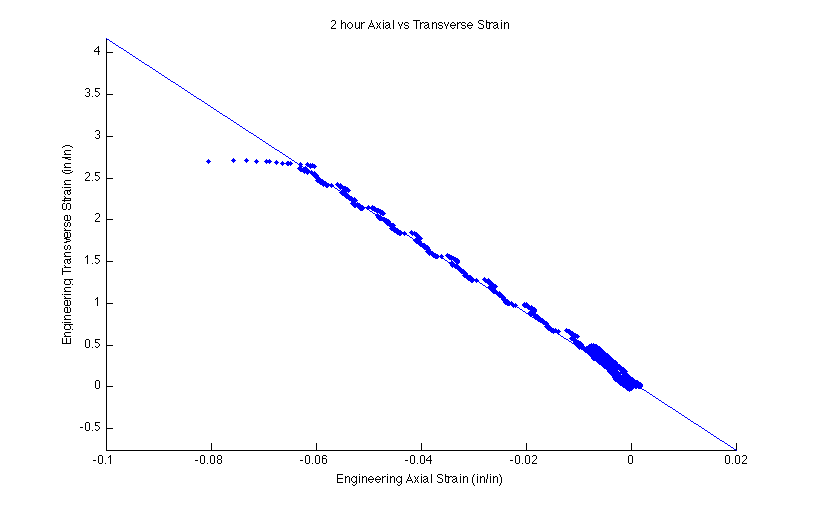
\includegraphics[width=1\textwidth]{2hour-strainvsstrain.png}
	\caption{Engineering axial vs. transverse strain for 2 hour treated aluminum}
	\label{fig:Figure10}
\end{figure}

\begin{figure}[H]
	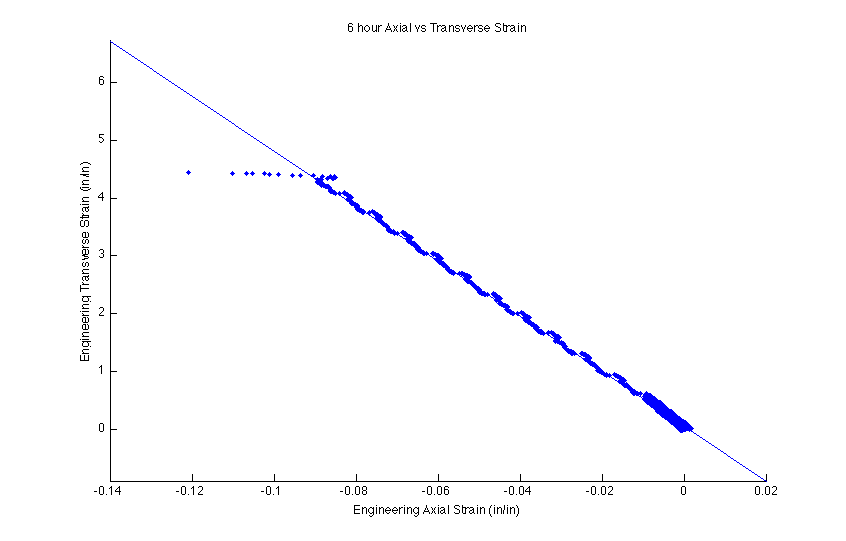
\includegraphics[width=1\textwidth]{6hour-strainvsstrain.png}
	\caption{Engineering axial vs. transverse strain for 6 hour treated aluminum}
	\label{fig:Figure11}
\end{figure}

\begin{figure}[H]
	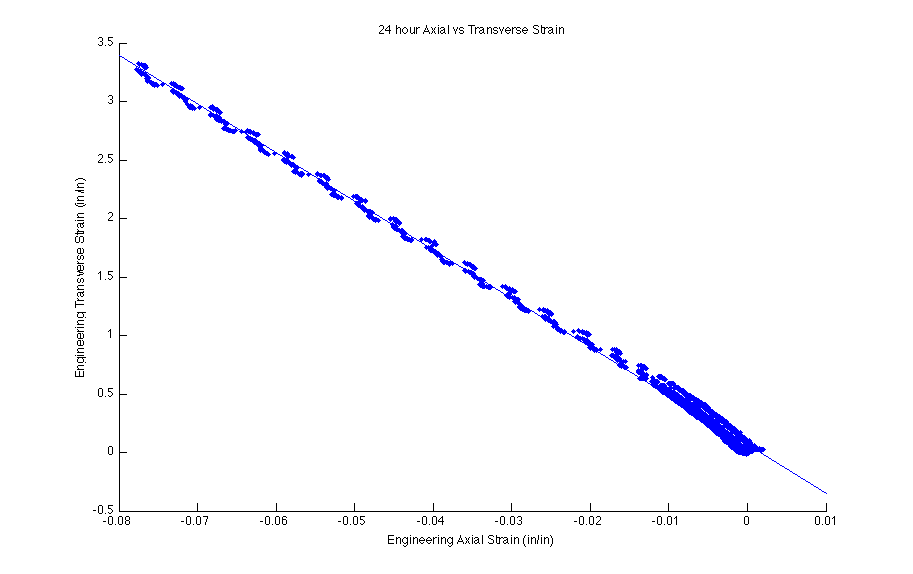
\includegraphics[width=1\textwidth]{24hour-strainvsstrain.png}
	\caption{Engineering axial vs. transverse strain for 24 hourtreated aluminum}
	\label{fig:Figure12}
\end{figure}

\begin{figure}[H]
	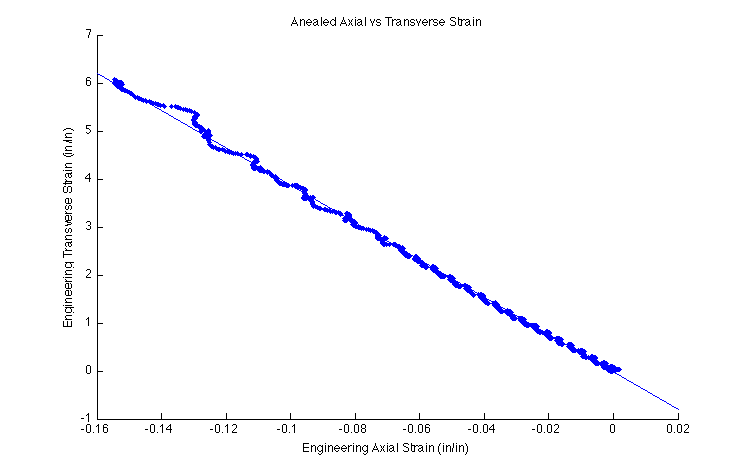
\includegraphics[width=1\textwidth]{anealed-strainvsstrain.png}
	\caption{Engineering axial vs. transverse strain for anealed aluminum}
	\label{fig:Figure13}
\end{figure}

With figures eight through thirteen used to find Poisson's ratio, the table with a numerical comparison is shown in figure fourteen.

\begin{figure}[H]
    \singlespacing
    \begin{tabular}{|p{2cm}|p{1.7cm}| p{1.7cm} | p{1.7cm} | p{1.7cm} | p{1.7cm} | p{1.7cm} |}
    \hline
    Treated Aluminum & Young's Modulus (ksi) & Poisson's Ratio (in/in) & 
    Yield stress at 0.2\% offset (ksi) & Ultimate tensile strength (ksi) & 
    Toughness (ksi-in) & Ductility (in/in) \\ \hline
    Untreated & 10523.265 & 0.249 & 50.610 & 68.385 & 10.275 & 0.185\\ \hline
    0.5 hour  &  8089.256 & 0.235 & 49.310 & 66.982 &  9.790 & 0.190\\ \hline
    2 hour    &  9115.904 & 0.243 & 49.720 & 67.601 & 10.774 & 0.215\\ \hline
    6 hour    &  6978.445 & 0.210 & 51.530 & 68.027 &  8.469 & 0.182\\ \hline
    24 hour   & 11446.964 & 0.241 & 61.630 & 67.522 &  3.011 & 0.067\\ \hline
    Anealed   & 14953.566 & 0.257 & 13.430 & 34.855 &  5.303 & 0.206\\ \hline
    \end{tabular}
    \caption{Comparison of properties of different treated aluminum}
\end{figure}\\
\doublespacing

There are clear differences between each of the treated aluminum specimen, each with different trade-offs in performance. 

Each of these specimen are treated by first mixing copper with aluminum at high temperatures (around 550 degrees Celsius), but each have been treated differently to perform differently. The untreated aluminum and copper is mixed at high temperature then rapidly dropped to room temperature, this is so quick the specimen is unable to form participate trapping the solution and making it super saturated. 

The aging process as seen in the time treated specimen, happens by cooling the material then reheating to around 190 degrees Celsius, or high enough for the atoms to have a phase transition and forms varying amounts of participates.

In the anealed case, the copper and aluminum mixture is brought up to extremely high temperatures to fully mix the solution, then the temperature is brought down very slowly. 

Based on the experimental results, the best temper to use for structural components in aircraft is either the two or six hour tempered aluminum. These are picked because of their high strength and toughness. Of the two tempered types, the two hour seems to be slightly better than the six hour treated, because of the higher toughness with only a relatively minimal impact to strength.

In this experiment, the materials have been hardened by impeding dislocation motion using two methods, solid solution and precipitate strengthening. The only one that was varied intentionally though-out was precipitate strengthening. There are two other known ways to increase the strength of materials: by work hardening, and by varying grain boundary parameters. By loading the specimen, or work hardening, this causes more dislocations that form and are entangled with each other, which then cause an increase in resistance to dislocation motion. This can be seen in the strain hardening phase where as the strain increases, the stress required to deform the material increases. 

The grain boundaries have a large effect on the hardening of the material. For instance, when decreasing the grain size in polycrystalline materials, the yielding strength increases greatly. These polycrystalline materials have different crystal orientations in different grains and each crystal structure has a disturbance at grain boundaries. When taking into account these polycrystals, the gross yield-strength is higher than single crystal structures by a factor of 50 percent. 

\section{Conclusion}
\doublespacing
In conclusion, the materials that were tested all displayed different properties based on how they were treated. The worst performing material ended up being the anealed aluminum, which displayed no augmented attributes. Under the assumption that the material would be used for the structure of an aircraft, the aluminum treated for two hours would provide the best trade-offs. In general, heat treating the specimen increased the strength, but toughness and other properties seemed to vary for each case. All of the specimen tested only varied the precipitate strengthening, but there are other ways to increase attributes of the materials that were not tested. 


\begin{thebibliography}{0}
\bibitem{notes} {\em ASE 324L Lab manual : The University of Texas at Austin Department of Aerospace Engineering}  2014.
\bibitem{notes} {\em ASE 324L Lecture 4 : The University of Texas at Austin Department of Aerospace Engineering}  2014.
\bibitem{notes} {\em ASE 324L Lecture 5 : The University of Texas at Austin Department of Aerospace Engineering}  2014.
\end{thebibliography}
\addcontentsline{toc}{section}{Bibliography}


\end{document}
